\documentclass[12pt, a4paper]{article}

% ── Codificación y lenguaje ──────────────────────────────────────────────────
\usepackage[utf8]{inputenc}
\usepackage[T1]{fontenc}
\usepackage[spanish]{babel}

% -- Hyperref
\usepackage{hyperref}
\hypersetup{
    colorlinks=true,
    linkcolor=blue,
    filecolor=magenta,      
    urlcolor=blue,
}

% ── Matemáticas ─────────────────────────────────────────────────────────────
\usepackage{amsmath, amssymb, amsthm}

% ── Diseño de página ────────────────────────────────────────────────────────
\usepackage[top=2.5cm, bottom=2.5cm, left=3cm, right=3cm]{geometry}
\usepackage{setspace}
\onehalfspacing

% ── Tipografía ──────────────────────────────────────────────────────────────
\usepackage{lmodern}
\usepackage{microtype}

% ── Colores y cajas ─────────────────────────────────────────────────────────
\usepackage[dvipsnames]{xcolor}
\usepackage{tcolorbox}
\usepackage{float}
\usepackage{siunitx}
\tcbuselibrary{skins, breakable}

% ── Tablas ──────────────────────────────────────────────────────────────────
\usepackage{booktabs}
\usepackage{array}

% ── Código fuente ───────────────────────────────────────────────────────────
\usepackage{listings}
\lstset{
  basicstyle=\ttfamily\small,
  backgroundcolor=\color{gray!10},
  frame=single,
  rulecolor=\color{gray!40},
  breaklines=true,
  inputencoding=utf8,
  extendedchars=true,
  literate=
    {á}{{\'a}}1 {é}{{\'e}}1 {í}{{\'i}}1 {ó}{{\'o}}1 {ú}{{\'u}}1
    {Á}{{\'A}}1 {É}{{\'E}}1 {Í}{{\'I}}1 {Ó}{{\'O}}1 {Ú}{{\'U}}1
    {ñ}{{\~n}}1 {Ñ}{{\~N}}1
    {±}{$\pm$}1 {·}{$\cdot$}1 {∓}{$\mp$}1,
}

% ── Cabeceras ───────────────────────────────────────────────────────────────
\usepackage{fancyhdr}
\pagestyle{fancy}
\fancyhf{}
\fancyhead[L]{\small\textit{Simulación Computacional de Flujo Incompresible}}
\fancyhead[R]{\small\thepage}
\renewcommand{\headrulewidth}{0.4pt}

% ── Definición de colores del documento ─────────────────────────────────────
\definecolor{azulTitulo}{RGB}{0, 70, 127}
\definecolor{verdeBox}{RGB}{0, 110, 80}
\definecolor{amarilloBox}{RGB}{255, 200, 0}

% ── Caja para ecuaciones destacadas ─────────────────────────────────────────
\newtcolorbox{ecbox}[1][]{
  colback=azulTitulo!5,
  colframe=azulTitulo!60,
  fonttitle=\bfseries,
  title=#1,
  breakable,
  arc=4pt,
}

% ── Caja de resumen / nota ───────────────────────────────────────────────────
\newtcolorbox{notabox}{
  colback=verdeBox!8,
  colframe=verdeBox!70,
  fonttitle=\bfseries,
  title=Resumen del sistema,
  arc=4pt,
}

%─────────────────────────────────────────────────────────────────────────────
\begin{document}

%─── Portada ─────────────────────────────────────────────────────────────────
\begin{titlepage}
  \centering
  \vspace*{2cm}
  {\color{azulTitulo}\rule{\linewidth}{1.5pt}}\par\vspace{0.4cm}
  {\color{azulTitulo}\rule{\linewidth}{0.4pt}}\par\vspace{1cm}

  {\Huge\bfseries\color{azulTitulo}
    Simulación Computacional}\par\vspace{0.4cm}
  {\LARGE\bfseries\color{azulTitulo}
    Flujo de Fluido Incompresible\\[0.3em]
    en Canal con Obstáculos}\par\vspace{1cm}

  {\color{azulTitulo}\rule{\linewidth}{0.4pt}}\par\vspace{0.3cm}
  {\color{azulTitulo}\rule{\linewidth}{1.5pt}}\par\vspace{2cm} 

  {\large Proyecto Final, Primer informe}\par\vspace{0.75cm}
    {\href{https://github.com/GG2R10/-streamfunction-vorticity-2d-nr}{Repositorio en GitHub}}\par\vspace{1.5cm}

    {\large Sebastián Calvo Carvajal - 2419118}\par\vspace{0.25cm}
    {\large Juan Esteban Arias Saldaña - 2417915}\par\vspace{0.25cm}
    {\large Yilver Julián Tello Larrahondo - 2110019}\par\vspace{0.5cm}

  {\large\today}\par
  \vfill
\end{titlepage}

%─── Índice ──────────────────────────────────────────────────────────────────
\tableofcontents
\newpage

%─────────────────────────────────────────────────────────────────────────────
\section{Introducción}
%─────────────────────────────────────────────────────────────────────────────

La hidrodinámica es un campo en donde constantemente nos encontramos con sistemas
de ecuaciones diferenciales no lineales de múltiples variables. Algunos de los
modelos matemáticos y específicamente sus soluciones nos permiten la predicción y
entendimiento de fenómenos físicos que luego pueden ser aplicados para la creación
de nuevas tecnologías, tales como la predicción meteorológica, el modelado oceánico
y el estudio del cambio climático, o para la prevención y cálculo de riesgo en
inundaciones, tsunamis y desastres hidrológicos.

Uno de este tipo de problemas es el \textbf{flujo de fluidos incompresibles}. El
objetivo de este proyecto es partir desde las bases matemáticas del fenómeno para
después adaptarlo y resolverlo de forma computacional mediante métodos numéricos,
la herramienta por excelencia para abordar problemas sin solución analítica cerrada.

%─────────────────────────────────────────────────────────────────────────────
\section{Descripción del Problema}
%─────────────────────────────────────────────────────────────────────────────

Se considera un canal de proporciones $10\!:\!1$ (horizontal$:$vertical) por el
que agua fluye de izquierda a derecha, con dos obstáculos sólidos que fuerzan la
desviación del fluido durante su recorrido. Las hipótesis del modelo son:

\begin{itemize}
  \item Dominio bidimensional $(x, y)$.
  \item Observación en un instante fijo (régimen estacionario).
  \item Fluido incompresible: densidad constante, $\partial\rho/\partial t = 0$.
  \item Viscosidad, presión y temperatura uniformes.
\end{itemize}

\subsection{Ecuación de continuidad}

Al ser incompresible, la ecuación de continuidad se reduce a:

\begin{equation}
  \frac{\partial v_x}{\partial x} + \frac{\partial v_y}{\partial y} = 0
\end{equation}

Esto garantiza la conservación de masa: todo el fluido que entra por un lado
debe salir por el otro; si choca con un obstáculo, alguna componente de su
velocidad cambia para poder desviarse.

\subsection{Ecuaciones de Navier-Stokes}

Las ecuaciones de Navier-Stokes son la segunda ley de Newton ($F = ma$)
adaptada a fluidos. En régimen estacionario y densidad constante, el balance
entre inercia, viscosidad y presión queda:

\begin{equation}
  (\mathbf{v} \cdot \nabla)\,\mathbf{v}
  = \nu\,\nabla^{2}\mathbf{v} - \frac{1}{\rho}\,\nabla P
\end{equation}

donde:
\begin{itemize}
  \item $\mathbf{v}$: campo de velocidades del fluido.
  \item $\nu$: viscosidad cinemática (resistencia del fluido al flujo).
  \item $\nu\,\nabla^{2}\mathbf{v}$: término de fricción interna (difusión viscosa).
  \item $\rho$: densidad del fluido.
  \item $\nabla P$: gradiente de presión (los fluidos se mueven de alta a baja presión).
\end{itemize}

Aun con estas simplificaciones, el sistema posee \textbf{tres incógnitas
entrelazadas} en cada punto: $v_x$, $v_y$ y $P$. Para reducir la complejidad se
reformula el problema en términos de dos nuevas variables: la \textbf{función de
corriente} $u$ y la \textbf{vorticidad} $w$.

\subsection{Función de corriente \texorpdfstring{$u$}{u}}

Se define una función escalar $u(x,y)$ cuyas curvas de nivel son precisamente
las \emph{streamlines} (líneas que siguen las partículas). Las componentes de la
velocidad se expresan como:

\begin{equation}
  v_x = \frac{\partial u}{\partial y}, \qquad
  v_y = -\frac{\partial u}{\partial x}
\end{equation}

Cualquier campo definido de esta forma satisface automáticamente la ecuación de
continuidad, sin necesidad de imponerla por separado.

\subsection{Vorticidad \texorpdfstring{$w$}{w}}

La vorticidad mide la rotación local del fluido alrededor de un punto. En 2D se
define como:

\begin{equation}
  w = \frac{\partial v_y}{\partial x} - \frac{\partial v_x}{\partial y}
\end{equation}

Si el flujo es perfectamente uniforme, $w = 0$. Cerca de una pared —donde existe
condición de no deslizamiento— aparece un gradiente de velocidad que genera
rotación local.

\subsection{Relación entre \texorpdfstring{$u$}{u} y \texorpdfstring{$w$}{w}: ecuación de Poisson}

Sustituyendo las expresiones de $v_x$ y $v_y$ en la definición de vorticidad:

\begin{equation}
  w = -\frac{\partial^{2} u}{\partial x^{2}} - \frac{\partial^{2} u}{\partial y^{2}}
\end{equation}

Reordenando se obtiene la \textbf{ecuación de Poisson}:

\begin{ecbox}[Ecuación de Poisson]
  \begin{equation}
    \nabla^{2} u = -w
    \label{eq:poisson}
  \end{equation}
\end{ecbox}

Esta ecuación relaciona la curvatura de las líneas de corriente con la rotación
local del fluido: si el fluido no gira, las líneas son suaves; si gira mucho,
las líneas se deforman.

\subsection{Ecuación de transporte de vorticidad}

La vorticidad es transportada por el fluido y se difunde por viscosidad. El
balance entre ambos efectos produce la \textbf{ecuación de transporte de
vorticidad}:

\begin{ecbox}[Ecuación de transporte de vorticidad]
  \begin{equation}
    \nabla^{2} w = R\!\left(
      \frac{\partial u}{\partial y}\frac{\partial w}{\partial x}
      - \frac{\partial u}{\partial x}\frac{\partial w}{\partial y}
    \right)
    \label{eq:transporte}
  \end{equation}
\end{ecbox}

\begin{itemize}
  \item \textbf{Lado izquierdo} $\nabla^{2}w$: difusión viscosa; la viscosidad
        suaviza y distribuye la vorticidad (análogo a la conducción de calor).
  \item \textbf{Lado derecho}: advección o transporte convectivo; el fluido
        arrastra la vorticidad consigo, dando lugar a remolinos y estelas.
\end{itemize}

El factor $R$ es el \textbf{número de Reynolds}:

\begin{equation}
  R = \frac{V_{0}\,h}{\nu}
\end{equation}

donde $V_{0}$ es la velocidad característica y $h$ el tamaño característico.
Un Reynolds pequeño ($R \ll 1$) produce flujo suave y estable; un Reynolds
grande ($R \gg 1$) tiende a la turbulencia.

\subsection{Ventaja de la reformulación}

\begin{notabox}
  Con el cambio de variables $\{v_x, v_y, P\} \to \{u, w\}$, la presión
  desaparece del cálculo. El sistema queda reducido a dos ecuaciones:
  \begin{enumerate}
    \item \textbf{Poisson} (lineal): $\nabla^{2}u = -w$
    \item \textbf{Transporte de vorticidad} (no lineal):
          $\nabla^{2}w = R\!\left(\dfrac{\partial u}{\partial y}
          \dfrac{\partial w}{\partial x}
          - \dfrac{\partial u}{\partial x}\dfrac{\partial w}{\partial y}\right)$
  \end{enumerate}
\end{notabox}

\subsection{¿Por qué aparece Poisson si el modelo es Navier-Stokes?}

Es importante aclarar que la ecuación de Poisson \textbf{no reemplaza} a
Navier-Stokes: es una \emph{consecuencia algebraica} de la reformulación
$\psi$--$\omega$, no una ley física independiente. El razonamiento es el
siguiente:

\begin{enumerate}
  \item Al definir $v_x = \partial u/\partial y$ y $v_y = -\partial u/\partial x$,
        la ecuación de continuidad (Ec.~1) queda satisfecha
        \textbf{automáticamente e idénticamente} para cualquier función $u$.
        Esto ya elimina una ecuación del sistema original sin haber tocado
        aún Navier-Stokes.
  \item La vorticidad es, por definición, una combinación de derivadas de
        $v_x$ y $v_y$. Al sustituir ahí las expresiones de $u$, se obtiene
        exactamente la ecuación de Poisson. Es decir, \textbf{Poisson es la
        definición de vorticidad reescrita en términos de $u$}, no una
        ecuación de balance de fuerzas nueva.
  \item La física de Navier-Stokes —inercia, viscosidad y gradiente de
        presión— no desaparece: se traslada íntegramente a la ecuación de
        transporte de vorticidad (Ec.~7), que se obtiene tomando el
        rotacional de Navier-Stokes precisamente para \textbf{cancelar el
        término de presión} $\nabla P$. Por eso la presión deja de ser una
        incógnita explícita del sistema.
\end{enumerate}

En consecuencia, el sistema \{Poisson, transporte de vorticidad\} es
\textbf{matemáticamente equivalente} a \{continuidad, Navier-Stokes\}, solo
que expresado en otras variables. Esta es la formulación \emph{streamfunction–vorticity},
un método estándar en CFD para problemas 2D incompresibles (véase~\cite{landau}),
que se adopta aquí precisamente porque reduce el número de incógnitas por
nodo de tres ($v_x, v_y, P$) a dos ($u, w$) sin perder información física.

%─────────────────────────────────────────────────────────────────────────────
\section{Discretización}
%─────────────────────────────────────────────────────────────────────────────

La computadora no puede manipular derivadas parciales ni espacios continuos.
Es necesario convertir el sistema a operaciones algebraicas sobre una
\textbf{malla finita} donde cada celda representa un punto del espacio.
Este proceso se denomina \textbf{discretización} y requiere dos pasos:

\begin{enumerate}
  \item Definir el espacio discreto (malla) con tamaño y número de puntos fijos.
  \item Transformar las ecuaciones diferenciales en relaciones algebraicas.
\end{enumerate}

\subsection{La malla}

La malla y los obstáculos se definen teniendo en cuenta dos criterios:
\begin{itemize}
  \item Que el número de iteraciones sea computacionalmente razonable.
  \item Que el número de Reynolds permanezca bajo, evitando soluciones
        inestables o caóticas que la discretización no podría capturar.
\end{itemize}

\begin{center}
\begin{tabular}{ll}
  \toprule
  \textbf{Elemento} & \textbf{Definición} \\
  \midrule
  Dominio   & 200 columnas $\times$ 20 filas \\
  Bloque 1  & cols.\ 0–8, filas 20–13 (arriba izquierda) \\
  Bloque 2  & cols.\ 90–98, filas 0-7 (abajo medio) \\
  \bottomrule
\end{tabular}
\end{center}

Los bloques son más anchos que altos para mantener el Reynolds bajo y garantizar
estabilidad numérica.

\subsection{Método de diferencias finitas}

El método de \textbf{diferencias finitas} aproxima derivadas mediante los valores
de los nodos vecinos. Las aproximaciones centradas empleadas son:

\textbf{Primera derivada:}
\begin{equation}
  \frac{\partial f}{\partial x}
  \approx \frac{f_{i+1,j} - f_{i-1,j}}{2h}
\end{equation}

\textbf{Segunda derivada:}
\begin{equation}
  \frac{\partial^{2} f}{\partial x^{2}}
  \approx \frac{f_{i+1,j} - 2f_{i,j} + f_{i-1,j}}{h^{2}}
\end{equation}

donde $h = 1$ es el espaciado entre nodos e $i, j$ son los índices del nodo
en la malla.

\subsection{Ecuaciones discretizadas}

Aplicando diferencias finitas a ambas ecuaciones, se obtiene el sistema
$F(\mathbf{x}) = \mathbf{0}$ para cada nodo interior $(i,j)$:

\bigskip
\noindent\textbf{Ecuación 1 — Poisson (lineal):}

\begin{equation}
  F^{u}_{i,j}
  = u_{i+1,j} + u_{i-1,j} + u_{i,j+1} + u_{i,j-1} + w_{i,j} - 4u_{i,j}
  = 0
  \label{eq:disc_poisson}
\end{equation}

Esta ecuación es \emph{lineal}: ningún término multiplica incógnitas entre sí.

\bigskip
\noindent\textbf{Ecuación 2 — Transporte de vorticidad (no lineal):}

\begin{equation}
  \begin{aligned}
    F^{w}_{i,j}
    &= w_{i+1,j} + w_{i-1,j} + w_{i,j+1} + w_{i,j-1} - 4w_{i,j} \\
    &\quad - \frac{R}{4}\Big[
        \bigl(u_{i,j+1} - u_{i,j-1}\bigr)\bigl(w_{i+1,j} - w_{i-1,j}\bigr) \\
    &\qquad\qquad - \bigl(u_{i+1,j} - u_{i-1,j}\bigr)\bigl(w_{i,j+1} - w_{i,j-1}\bigr)
    \Big] = 0
  \end{aligned}
  \label{eq:disc_vort}
\end{equation}

El factor $R/4$ proviene de las dos diferencias centrales multiplicadas: cada
una aporta $\tfrac{1}{2h}$ y, con $h=1$, resulta $\tfrac{1}{4}$. Los productos
de incógnitas (e.g., $(u_{i,j+1} - u_{i,j-1})(w_{i+1,j} - w_{i-1,j})$)
introducen la \textbf{no linealidad} que impide resolver el sistema de forma directa.

Tras la discretización, el sistema completo tiene la forma:
\begin{equation}
  F(\mathbf{x}) = \mathbf{0}
\end{equation}
donde $\mathbf{x}$ contiene todos los valores de $u$ y $w$ en cada nodo interior.

%─────────────────────────────────────────────────────────────────────────────
\section{Solución del Sistema de Ecuaciones No Lineales}
%─────────────────────────────────────────────────────────────────────────────

El sistema discretizado \(F(\mathbf{x}) = \mathbf{0}\) involucra \(2N_{\text{act}}\) incógnitas. Para que la resolución sea viable, la malla se clasifica en seis tipos de nodo según su rol físico:

\begin{itemize}
    \item \textbf{Activos} (\texttt{FREE}, \texttt{BC\_WALL}, \texttt{WALL}, \texttt{OUTLET}): son las verdaderas incógnitas; Newton-Raphson las actualiza en cada iteración.
    \item \textbf{Fijos} (\texttt{INLET}, \texttt{SOLID}): sus valores están impuestos \emph{a priori}. No se actualizan y \textbf{no generan columnas en la Jacobiana}, solo contribuyen como términos constantes al residuo.
\end{itemize}

El vector de estado se empaqueta como
\[
\mathbf{x} = \bigl[\,\psi_0,\dots,\psi_{N_{\text{act}}-1},\;
                \omega_0,\dots,\omega_{N_{\text{act}}-1}\,\bigr]^{\!\top},
\]
y una tabla \texttt{node\_id} permite la correspondencia \(O(1)\) entre las coordenadas de malla \((i,j)\) y el índice en \(\mathbf{x}\).

Entre las partes destacadas de la implementación destacan:

\begin{itemize}
    \item \textbf{Condición de Thom en paredes}: los nodos adyacentes a superficies sólidas (\texttt{BC\_WALL}, \texttt{WALL}) no resuelven la ecuación de transporte, sino una relación lineal
    \[
    \omega_{\text{pared}} + \frac{2}{h^{2}}\bigl(\psi_{\text{interior}} - \psi_{\text{sólido}}\bigr) = 0,
    \]
    que genera entradas triviales en la Jacobiana: \(\partial F^\omega/\partial\omega_{\text{pared}} = 1\) y \(\partial F^\omega/\partial\psi_{\text{interior}} = 2/h^{2}\).

    \item \textbf{Condición de salida Neumann}: en \texttt{OUTLET} se impone gradiente nulo (\(\psi_{N_x,j} - \psi_{N_x-1,j}=0\), análogo para \(\omega\)). Esto acopla el nodo de frontera con su vecino interior, por lo que se trata como activo y genera filas con coeficientes \(+1\) y \(-1\) en \(J\).
\end{itemize}

\medskip
\noindent\textbf{La matriz Jacobiana dispersa (sparse).}

Cada ecuación del sistema solo conecta el nodo consigo mismo y con un máximo de 4 vecinos, de modo que la Jacobiana
\[
J \in \mathbb{R}^{2N_{\text{act}} \times 2N_{\text{act}}}
\]

contiene del orden de \(10\,N_{\text{act}}\) entradas no nulas frente a \((2N_{\text{act}})^{2}\) posibles. Para una malla de \(200 \times 20\) nodos, la densidad es inferior al \(0.1\,\text{\%}\). Almacenarla en formato denso sería inviable; por ello se emplea el formato \textbf{CSR} (\emph{Compressed Sparse Row}) y el sistema lineal \(J\,\Delta\mathbf{x} = -F\) se resuelve con \texttt{scipy.sparse.linalg.spsolve}, cuyo coste escala con el número de entradas no nulas y no con la dimensión total de la matriz. Con estas implementaciones podemos ir obteniendo poco a poco convergencia en el sistema y una solución. 


\subsection{Cálculo de la Matriz Jacobiana}
\label{ssec:jacobiana}

La Jacobiana es la matriz de derivadas parciales:

\begin{equation}
  J_{ij} = \frac{\partial F_{i}}{\partial x_{j}}
\end{equation}

El vector $\mathbf{x}$ tiene tamaño $2\cdot N_{\text{interior}}$, organizado
con todos los valores de $u$ seguidos de todos los de $w$:

\begin{equation}
  \mathbf{x} = \bigl[\ldots,\, u_{i,j},\, \ldots,\, w_{i,j},\, \ldots\bigr]
\end{equation}

Esto confiere a la Jacobiana una \textbf{estructura en bloques} $2 \times 2$:

\begin{equation}
  J = \begin{bmatrix} A & B \\ C & D \end{bmatrix}
\end{equation}

\bigskip
\noindent\textbf{Bloque A — $\partial F^{u}/\partial u$ (lineal, constante):}

\begin{center}
\begin{tabular}{lc}
  \toprule
  \textbf{Derivada} & \textbf{Valor} \\
  \midrule
  $\partial F^{u}_{i,j}/\partial u_{i,j}$        & $-4$ \\
  $\partial F^{u}_{i,j}/\partial u_{i\pm1,j}$    & $+1$ \\
  $\partial F^{u}_{i,j}/\partial u_{i,j\pm1}$    & $+1$ \\
  Todos los demás                                 & $0$  \\
  \bottomrule
\end{tabular}
\end{center}

Es el Laplaciano discreto. Como $F^{u}$ es lineal, este bloque es
\emph{constante} y no varía entre iteraciones.

\bigskip
\noindent\textbf{Bloque B — $\partial F^{u}/\partial w$ (identidad):}

\begin{center}
\begin{tabular}{lc}
  \toprule
  \textbf{Derivada} & \textbf{Valor} \\
  \midrule
  $\partial F^{u}_{i,j}/\partial w_{i,j}$ & $+1$ \\
  Todos los demás                          & $0$  \\
  \bottomrule
\end{tabular}
\end{center}

Dado que $F^{u}$ solo depende de $w$ a través del término $+w_{i,j}$, este
bloque es una matriz identidad.

\bigskip
\noindent\textbf{Bloque C — $\partial F^{w}/\partial u$ (no lineal, varía en cada iteración):}

Derivando el término convectivo respecto a los valores de $u$:

\begin{align}
  \frac{\partial F^{w}_{i,j}}{\partial u_{i,j+1}} &= -\frac{R}{4}(w_{i+1,j} - w_{i-1,j}) \\[4pt]
  \frac{\partial F^{w}_{i,j}}{\partial u_{i,j-1}} &= +\frac{R}{4}(w_{i+1,j} - w_{i-1,j}) \\[4pt]
  \frac{\partial F^{w}_{i,j}}{\partial u_{i+1,j}} &= +\frac{R}{4}(w_{i,j+1} - w_{i,j-1}) \\[4pt]
  \frac{\partial F^{w}_{i,j}}{\partial u_{i-1,j}} &= -\frac{R}{4}(w_{i,j+1} - w_{i,j-1})
\end{align}

Estas entradas \textbf{dependen del estado actual de $w$} y se recalculan en
cada iteración de Newton.

\bigskip
\noindent\textbf{Bloque D — $\partial F^{w}/\partial w$ (no lineal, varía en cada iteración):}

\begin{align}
  \frac{\partial F^{w}_{i,j}}{\partial w_{i,j}}   &= -4 \\[4pt]
  \frac{\partial F^{w}_{i,j}}{\partial w_{i+1,j}} &= 1 - \frac{R}{4}(u_{i,j+1} - u_{i,j-1}) \\[4pt]
  \frac{\partial F^{w}_{i,j}}{\partial w_{i-1,j}} &= 1 + \frac{R}{4}(u_{i,j+1} - u_{i,j-1}) \\[4pt]
  \frac{\partial F^{w}_{i,j}}{\partial w_{i,j+1}} &= 1 + \frac{R}{4}(u_{i+1,j} - u_{i-1,j}) \\[4pt]
  \frac{\partial F^{w}_{i,j}}{\partial w_{i,j-1}} &= 1 - \frac{R}{4}(u_{i+1,j} - u_{i-1,j})
\end{align}

Estas entradas \textbf{dependen del estado actual de $u$} y también se
recalculan en cada iteración.

\bigskip

Dado que cada ecuación solo involucra el nodo actual y sus 4 vecinos inmediatos,
la Jacobiana es \textbf{sparse} (dispersa): enorme en dimensiones pero con casi
todas sus entradas en cero. Ello hace al problema computacionalmente tratable.

El resumen de entradas no nulas por nodo interior $(i,j)$ es:

\begin{lstlisting}
De F^u:  u_{i,j}(-4),  u_vecinos(+1),  w_{i,j}(+1)          
->  5 entradas

De F^w:  w_{i,j}(-4),  w_vecinos(1 +/- R/4*Delta_u),
         u_{i,j+-1}(-/+ R/4*Delta_w),  u_{i+-1,j}(+/- R/4*Delta_w)
->  9 entradas
\end{lstlisting}

Los bloques $A$ y $B$ son constantes; los bloques $C$ y $D$ son no lineales
y deben actualizarse en cada paso de Newton-Raphson.

\subsection{Parámetros y condiciones de frontera}

Las condiciones de frontera definen el comportamiento del fluido en los bordes
del dominio y sobre las superficies de los obstáculos. Son esenciales para que
el sistema tenga una solución física.

Se parte de $V_{0} = 1$, $h = 1$ y $\nu = 1$, dando $R = V_{0}h/\nu = 1$.

\bigskip
\noindent\textbf{¿Por qué fijar $R$ y no dejarlo libre según su definición?}

El valor de $R$ no se escoge de forma arbitraria, sino que resulta de
\textbf{adimensionalizar} el problema. La definición $R = V_0 h/\nu$
depende de tres cantidades dimensionales que, en una simulación numérica sin
un fluido ni un experimento físico concretos de referencia, no tienen una
escala natural propia. La práctica estándar —y la que se sigue aquí— es
tomar $V_0$ y $h$ como las \textbf{escalas de referencia} de velocidad y
longitud del problema (de ahí $V_0 = h = 1$), dejando a $R$ como el
\textbf{único parámetro de control libre} del sistema, ajustable a través
de $\nu$. Fijar las escalas de referencia no es lo mismo que fijar
arbitrariamente el fenómeno: $R$ sigue siendo una cantidad libre, solo que
se manipula indirectamente mediante $\nu$ en vez de mediante $V_0$ o $h$.

El valor final usado para reportar resultados ($Re = 2$,
Sección~\ref{sec:resultados}) tampoco es arbitrario: se alcanzó mediante una
\textbf{continuación gradual en Reynolds}, partiendo de un $R$ bajo e
incrementándolo poco a poco (ver la Sección~\ref{ssec:continuacion}), por dos
razones concretas:
\begin{itemize}
  \item Mantener el régimen \textbf{laminar}, coherente con la hipótesis de
        flujo estacionario adoptada en la Sección~2.
  \item Garantizar la \textbf{estabilidad numérica} de Newton-Raphson: un
        salto directo a un $R$ alto haría que el término convectivo no
        lineal dominara desde la primera iteración, alejando la
        aproximación inicial de la región de convergencia del método.
\end{itemize}

\bigskip
\noindent\textbf{Inicialización general:}

Todos los nodos se inicializan con vorticidad nula y función de corriente
proporcional a la posición vertical, reflejando un flujo uniforme de entrada:

\begin{equation}
  u_{i,j} = j\cdot V_{0}, \qquad w_{i,j} = 0
\end{equation}

\bigskip
\noindent\textbf{Borde superior (flujo superior abierto):}

Flujo libre y uniforme; vorticidad nula. El Bloque~1 ocupa las columnas 0--8 y
llega hasta la fila superior ($j = N_y$), por lo que esta condición se aplica
únicamente en las columnas $i \geq 9$:

\begin{equation}
  u_{i,\,N_y} = u_{i,\,N_y-1} + V_{0}\cdot h, \qquad
  w_{i,\,N_y-1} = 0 \quad (i \geq 9)
\end{equation}

\bigskip
\noindent\textbf{Borde izquierdo (entrada):}

El Bloque~1 está pegado al borde izquierdo (cols.\ 0--8), de modo que la
condición de entrada libre solo aplica en las filas por debajo del bloque
($j < 13$). En las filas ocupadas por el bloque se impone directamente
$u = 0$ (ver condición de obstáculos):

\begin{equation}
  u_{1,j} = u_{0,j}, \qquad w_{0,j} = 0 \quad (j < 13)
\end{equation}

\bigskip
\noindent\textbf{Borde inferior (base del canal):}

En zonas sin obstáculo, la base es una pared con condición de no deslizamiento.
El Bloque~2 ocupa las filas 0--7 en las columnas 90--98, por lo que en esas
columnas la condición de pared queda reemplazada por la condición de obstáculo:

\begin{equation}
  u_{i,0} = 0, \qquad w_{i,0} = 0
  \quad \text{(cols.\ } i \notin [90,\,98]\text{)}
\end{equation}

\bigskip
\noindent\textbf{Borde derecho (salida):}

Condición de salida libre (extrapolación desde el interior):

\begin{equation}
  u_{N_x,\,j} = u_{N_x-1,\,j}, \qquad w_{N_x,\,j} = w_{N_x-1,\,j}
\end{equation}

\bigskip
\noindent\textbf{Obstáculos:}

\begin{itemize}
  \item \textbf{Bloque 1:} cols.\ 0--8, filas 13--20 (esquina superior izquierda).
        Al estar pegado tanto al borde superior como al borde izquierdo, solo
        expone dos caras al fluido: la \emph{cara inferior} y la \emph{cara derecha}.
  \item \textbf{Bloque 2:} cols.\ 90--98, filas 0--7 (zona inferior central).
        Al estar pegado al borde inferior, expone tres caras al fluido:
        \emph{cara frontal} (izquierda), \emph{cara trasera} (derecha) y
        \emph{cara superior}.
\end{itemize}

Sobre todas las superficies expuestas se aplica la condición de no deslizamiento
($u = 0$). La vorticidad en cada pared se aproxima con diferencias finitas hacia
el interior del fluido:

\begin{itemize}

  \item \textbf{Cara frontal / izquierda}
        (primera columna del bloque, para cada fila $j$ interior al bloque):
  \begin{equation}
    w_{\text{front},\,j} = -\frac{2\,u_{\text{front}-1,\,j}}{h^{2}}
  \end{equation}

  \item \textbf{Cara trasera / derecha}
        (última columna del bloque, para cada fila $j$ interior al bloque):
  \begin{equation}
    w_{\text{back},\,j} = -\frac{2\,u_{\text{back}+1,\,j}}{h^{2}}
  \end{equation}

  \item \textbf{Cara superior}
        (fila más alta del bloque, para cada columna $i$ interior al bloque;
        aplica al Bloque~2 y a la cara inferior del Bloque~1 vista desde el fluido):
  \begin{equation}
    w_{i,\,\text{top}-1} = -\frac{2\,u_{i,\,\text{top}}}{h^{2}}
  \end{equation}

  \item \textbf{Cara inferior}
        (fila más baja del bloque, para cada columna $i$ interior al bloque;
        aplica únicamente al Bloque~1, que no toca el borde inferior):
  \begin{equation}
    w_{i,\,\text{bot}+1} = -\frac{2\,u_{i,\,\text{bot}}}{h^{2}}
  \end{equation}

  \item \textbf{Interior y bordes del bloque:} $u = 0$ en toda la extensión
        del obstáculo.

\end{itemize}

Estas condiciones garantizan que el fluido no penetre ni se deslice sobre los
obstáculos, y que la vorticidad en sus paredes sea consistente con el campo de
corriente del fluido adyacente.

\subsection{Algoritmo de Newton-Raphson}

Con $F(\mathbf{x})$ y $J(\mathbf{x})$ ya definidos, falta describir cómo se
usan en la práctica para llegar a la solución. La idea de Newton-Raphson es
simple: partiendo de una aproximación $\mathbf{x}^{(k)}$, se resuelve el
sistema lineal

\begin{ecbox}[Paso de Newton-Raphson]
  \begin{equation}
    J(\mathbf{x}^{(k)})\,\Delta\mathbf{x} = -F(\mathbf{x}^{(k)})
    \label{eq:newton_lineal}
  \end{equation}
\end{ecbox}

y se actualiza la aproximación como $\mathbf{x}^{(k+1)} = \mathbf{x}^{(k)} +
\Delta\mathbf{x}$. Como $F$ es no lineal, $\Delta\mathbf{x}$ no lleva
directamente a la solución exacta; por eso el proceso se repite, recalculando
$F$ y $J$ en cada iteración, hasta que el residuo sea suficientemente pequeño.
En la implementación (\texttt{newton\_raphson} en \texttt{simulacion.py}) el
criterio de convergencia es

\begin{equation}
  \|F(\mathbf{x}^{(k)})\|_2 < \text{tol}, \qquad \text{tol} = 10^{-7},
\end{equation}

con un máximo de 50 iteraciones por valor de $R$. En cada iteración se arma
$J$ en formato sparse (Sección~4) y se resuelve la Ec.~\eqref{eq:newton_lineal}
con \texttt{scipy.sparse.linalg.spsolve}, que aprovecha la dispersión de $J$
para factorizarla eficientemente en lugar de invertirla explícitamente.

\subsubsection{Backtracking: por qué el paso completo no siempre funciona}

Newton-Raphson asume que $\Delta\mathbf{x}$ es una buena dirección de mejora,
pero no garantiza que dar el \emph{paso completo} ($\mathbf{x}^{(k)} +
\Delta\mathbf{x}$) realmente reduzca el residuo. Con un sistema tan no lineal
como el de transporte de vorticidad, un paso completo puede sobrepasar la
solución y hacer que $\|F\|$ \textbf{aumente} en vez de disminuir, especialmente
en las primeras iteraciones cuando la aproximación inicial está lejos de la
solución real.

Para evitar esto se introduce un factor de amortiguación $\alpha \in (0,1]$,
de modo que la actualización real es

\begin{equation}
  \mathbf{x}^{(k+1)} = \mathbf{x}^{(k)} + \alpha\,\Delta\mathbf{x}.
\end{equation}

El algoritmo de \textbf{backtracking} (búsqueda de línea) implementado
funciona así:

\begin{enumerate}
  \item Se prueba primero $\alpha = 1$ (el paso completo de Newton).
  \item Se evalúa $\|F\|$ con ese $\alpha$. Si mejora respecto al residuo
        actual, se acepta y se pasa a la siguiente iteración de Newton.
  \item Si no mejora, se reduce el paso a la mitad ($\alpha \to \alpha/2$) y
        se repite la prueba, hasta un máximo de 40 reducciones o hasta que
        $\alpha$ sea menor que $10^{-12}$ (\texttt{alpha\_min}), momento en
        el cual se considera que la búsqueda de línea fracasó.
\end{enumerate}

En otras palabras, el método siempre intenta primero el paso ideal de
Newton-Raphson, y solo lo acorta cuando ese paso resulta contraproducente.
Esto conserva la velocidad de convergencia de Newton cuando el sistema se
comporta bien, pero evita que un paso demasiado agresivo tumbe la iteración
cuando el sistema aún está lejos de converger.

Como salvaguarda adicional, si en algún punto el residuo crece por un factor
mayor a 10 respecto a la iteración anterior, el solver interpreta esto como
una divergencia y detiene el intento para ese valor de $R$, en vez de seguir
iterando sin sentido.

\subsubsection{Continuación en Reynolds}
\label{ssec:continuacion}

Incluso con backtracking, arrancar Newton-Raphson directamente en el $R$
deseado (por ejemplo $R=2$) desde la condición inicial de flujo uniforme
(Ec.~26) puede fallar: el término convectivo no lineal de la ecuación de
transporte de vorticidad ya tiene demasiado peso desde el principio, y la
aproximación inicial queda lejos de la región donde Newton-Raphson converge.

La solución adoptada es una \textbf{continuación en Reynolds}: en vez de
resolver una sola vez para el $R$ objetivo, se resuelve una secuencia
creciente de valores de $R$, usando la solución convergida de un paso como
punto de partida del siguiente:

\begin{equation}
  R_0 = 0.01 \;\to\; R_1 \;\to\; \dots \;\to\; R_n = R_{\text{objetivo}}.
\end{equation}

Como el primer $R_0$ es muy pequeño, el sistema es casi lineal (el término
convectivo pesa poco) y Newton-Raphson converge fácilmente desde el flujo
uniforme. Cada paso siguiente parte de una solución ya cercana a la correcta
para el nuevo $R$, así que el paso completo de Newton vuelve a ser efectivo
la mayoría de las veces. La función \texttt{re\_continuation} arma esta
secuencia de forma más fina cuanto más alto es el $R$ objetivo (más pasos
intermedios entre $R=20$ y $R=50$, por ejemplo, que entre $R=0$ y $R=1$),
ya que la no linealidad se vuelve más fuerte a medida que $R$ crece.

Si a pesar de la continuación un paso de $R$ falla en converger, el algoritmo
no se detiene de inmediato: \textbf{subdivide} el intervalo entre el último
$R$ convergido y el que falló en pasos más pequeños, y reintenta. Solo si esa
subdivisión también falla se reporta una solución parcial hasta el último $R$
alcanzado con éxito. En la práctica, para $Re=2$ (el caso reportado en la
Sección~\ref{sec:resultados}) esta continuación converge sin necesidad de
subdivisiones adicionales.

\begin{notabox}
  En resumen, la solución del sistema no lineal combina tres ingredientes:
  \begin{enumerate}
    \item \textbf{Newton-Raphson}: linealiza el sistema en cada iteración
          resolviendo $J\,\Delta\mathbf{x} = -F$ con un solver sparse.
    \item \textbf{Backtracking}: amortigua el paso de Newton cuando el paso
          completo empeoraría el residuo, probando $\alpha = 1, \tfrac12,
          \tfrac14,\dots$
    \item \textbf{Continuación en Reynolds}: evita arrancar directamente en
          el $R$ difícil, resolviendo una secuencia creciente de problemas
          más fáciles que van "calentando" la solución hasta el $R$ objetivo.
  \end{enumerate}
  Sin estos tres elementos combinados, el sistema no lineal —altamente
  sensible al valor de $R$— habría sido extremadamente inestable de resolver
  directamente, tal como se anticipa en los comentarios finales del informe.
\end{notabox}

%─────────────────────────────────────────────────────────────────────────────
\section{Esquema \emph{upwind} para el término convectivo}
\label{sec:upwind}
%─────────────────────────────────────────────────────────────────────────────

Al intentar subir el número de Reynolds más allá de valores modestos, la
discretización centrada del término convectivo (Ec.~\eqref{eq:disc_vort})
comenzó a producir soluciones con oscilaciones no físicas. Esta sección
explica el origen del problema y el cambio de esquema que se adoptó para
eliminarlo.

\subsection{Limitación de las diferencias centradas: el Reynolds de celda}

Conviene reescribir el término convectivo en función de las velocidades
locales del fluido, obtenidas de la función de corriente por diferencias
centradas:
\begin{equation}
  v_x = \frac{u_{i,j+1} - u_{i,j-1}}{2h}, \qquad
  v_y = -\frac{u_{i+1,j} - u_{i-1,j}}{2h}.
\end{equation}

Con esta notación, los coeficientes del bloque $D$ de la Jacobiana
(Sección~\ref{ssec:jacobiana}) que acompañan a los vecinos de $w$ quedan:
\begin{equation}
  \frac{\partial F^{w}_{i,j}}{\partial w_{i\pm1,j}}
    = 1 \mp \frac{R\,h}{2}\,v_x, \qquad
  \frac{\partial F^{w}_{i,j}}{\partial w_{i,j\pm1}}
    = 1 \mp \frac{R\,h}{2}\,v_y.
\end{equation}

Para que estos coeficientes \emph{no cambien de signo} se necesita que el
llamado \textbf{Reynolds de celda} sea pequeño:
\begin{equation}
  \mathrm{Re}_{\text{celda}} = R\,|v|\,h < 2.
\end{equation}

Mientras esa condición se cumple, la matriz del sistema es una
\emph{M-matriz} (diagonal dominante con vecinos de signo uniforme) y la
solución discreta respeta el \textbf{principio del máximo}: la vorticidad no
puede desarrollar extremos espurios en el interior del dominio. Pero cuando
$\mathrm{Re}_{\text{celda}}$ supera el umbral —por ejemplo a $Re = 10$ en la
malla de $200\times20$, donde llega a valores de orden $50$ en buena parte
del canal— los coeficientes de los vecinos cambian de signo, la estructura de
M-matriz se pierde y aparecen \textbf{oscilaciones espurias}: vorticidad de
signo alternado tipo ``tablero de ajedrez'', saltos bruscos en las líneas de
corriente y velocidades infladas.

Es importante subrayar que Newton--Raphson \emph{sí converge} en ese caso:
converge a la solución exacta del sistema discreto, pero es el propio sistema
discreto el que está mal planteado. El problema no es del método iterativo,
sino de la discretización.

\subsection{La discretización \emph{upwind}}

La solución adoptada es clásica en CFD: aproximar las derivadas de $w$ del
término convectivo con diferencias \emph{unilaterales} tomadas ``río
arriba'' (\emph{upwind}), es decir, del lado desde el que viene el fluido
según el signo de la velocidad local:

\begin{ecbox}[Derivadas upwind de la vorticidad]
  \begin{equation}
    \left.\frac{\partial w}{\partial x}\right|_{i,j}^{\text{up}} =
    \begin{cases}
      \dfrac{w_{i,j} - w_{i-1,j}}{h} & \text{si } v_x \geq 0
        \quad\text{(hacia atrás)},\\[10pt]
      \dfrac{w_{i+1,j} - w_{i,j}}{h} & \text{si } v_x < 0
        \quad\text{(hacia adelante)},
    \end{cases}
  \end{equation}
  y de forma análoga para $\partial w/\partial y$ según el signo de $v_y$.
\end{ecbox}

La ecuación discreta de transporte de vorticidad en los nodos \texttt{FREE}
pasa a ser
\begin{equation}
  F^{w}_{i,j}
  = w_{i+1,j} + w_{i-1,j} + w_{i,j+1} + w_{i,j-1} - 4\,w_{i,j}
  - R\,h^{2}\left(
      v_x \left.\frac{\partial w}{\partial x}\right|^{\text{up}}
    + v_y \left.\frac{\partial w}{\partial y}\right|^{\text{up}}
    \right) = 0,
  \label{eq:disc_vort_upwind}
\end{equation}
que reemplaza a la Ec.~\eqref{eq:disc_vort}. El resto del sistema —la
ecuación de Poisson, las condiciones de Thom, la salida Neumann— no se
modifica. Físicamente el esquema es coherente con la naturaleza de la
advección: la información de la vorticidad viaja \emph{con} el fluido, así
que el nodo debe ``mirar'' hacia el lado del que viene el flujo.

\subsection{Efecto sobre la Jacobiana}

Con el esquema upwind, las derivadas del bloque $D$ se convierten en
\begin{align}
  \frac{\partial F^{w}_{i,j}}{\partial w_{i,j}}
    &= -4 - R\,h\left(|v_x| + |v_y|\right),\\[4pt]
  \frac{\partial F^{w}_{i,j}}{\partial w_{\text{río arriba}}}
    &= 1 + R\,h\,|v_x| \quad(\text{o } |v_y|),\\[4pt]
  \frac{\partial F^{w}_{i,j}}{\partial w_{\text{río abajo}}}
    &= 1.
\end{align}

Los coeficientes de los vecinos son ahora \textbf{siempre positivos} y la
diagonal se \textbf{refuerza} en lugar de debilitarse: la estructura de
M-matriz —y con ella el principio del máximo discreto— se conserva para
\emph{cualquier} valor de $\mathrm{Re}_{\text{celda}}$. Además, el mejor
condicionamiento de la matriz hace que Newton--Raphson converja en menos
iteraciones a Reynolds alto. El bloque $C$ ($\partial F^{w}/\partial u$)
también cambia: las derivadas de $w$ que lo acompañan pasan a ser las
unilaterales del esquema. La Jacobiana analítica resultante se verificó
contra diferencias finitas, con discrepancias del orden de $10^{-8}$.

\subsection{Ventajas y compromisos}

El precio de la estabilidad incondicional es la precisión:

\begin{itemize}
  \item \textbf{Orden de precisión}: la derivada unilateral es de primer
        orden, $O(h)$, frente al $O(h^{2})$ del esquema centrado.
  \item \textbf{Difusión numérica}: el error de truncamiento del upwind actúa
        como una viscosidad artificial proporcional a $|v|\,h$, que suaviza
        los gradientes finos y sub-predice la intensidad pico de la
        vorticidad y de las recirculaciones. En la práctica, el ``Reynolds
        efectivo'' resuelto es algo menor que el nominal.
  \item \textbf{No diferenciabilidad en $v = 0$}: el cambio de rama del
        esquema introduce un punto anguloso en $F$; Newton--Raphson lo tolera
        bien, aunque puede costar alguna iteración extra cerca de puntos de
        estancamiento.
\end{itemize}

Como referencia del efecto estabilizador: a $Re = 10$, con el esquema
centrado la vorticidad se disparaba al rango $[-31.7,\,20.2]$ con
oscilaciones de signo alternado, mientras que con upwind se mantiene en
$[-6.3,\,5.4]$ sin oscilaciones.

\begin{center}
\begin{tabular}{lcc}
  \toprule
   & \textbf{Centrado} & \textbf{Upwind} \\
  \midrule
  Orden de precisión (convección) & $O(h^{2})$ & $O(h)$ \\
  Estabilidad & solo si $\mathrm{Re}_{\text{celda}} < 2$ & incondicional \\
  Difusión numérica & nula & $\propto |v|\,h$ \\
  $Re$ alcanzable (malla $200\times20$) & bajo ($\approx 2$) & moderado ($\geq 10$) \\
  \bottomrule
\end{tabular}
\end{center}

%─────────────────────────────────────────────────────────────────────────────
\section{Malla reducida y splines cúbicos naturales}
\label{sec:spline}
%─────────────────────────────────────────────────────────────────────────────

La última mejora incorporada ataca el \textbf{costo computacional}: en lugar
de resolver el sistema no lineal directamente sobre la malla completa de
$200\times20$, se resuelve sobre una malla más gruesa y la solución se lleva
de vuelta al tamaño original interpolando con \textbf{splines cúbicos
naturales}.

\subsection{Motivación}

Cada iteración de Newton--Raphson debe evaluar el residuo $F$, ensamblar la
Jacobiana sparse y resolver $J\,\Delta\mathbf{x} = -F$; además, el
\emph{backtracking} vuelve a evaluar $F$ varias veces por iteración, y la
continuación en Reynolds repite todo el proceso para decenas de valores de
$R$. Todo ese trabajo escala con el número de nodos activos. Al reducir la
malla por un factor \texttt{FACTOR} en cada dirección, el número de nodos
—y con él el costo de cada una de esas operaciones— cae aproximadamente en
un factor $\texttt{FACTOR}^{2}$ (con $\texttt{FACTOR}=2$: de $2N_{\text{act}}
\approx 8\,000$ grados de libertad a unos $2\,100$).

\subsection{La malla gruesa equivalente}

Reducir la malla no es solo quitar nodos: si el espaciado se dejara igual,
el canal se encogería. La idea es repartir el mismo dominio físico entre
menos nodos, dividiendo el número de celdas y agrandando el espaciado en la
misma proporción:
\begin{equation}
  N_x' = \frac{N_x}{\texttt{FACTOR}}, \qquad
  N_y' = \frac{N_y}{\texttt{FACTOR}}, \qquad
  h' = \texttt{FACTOR}\cdot h.
\end{equation}
Como $N_x'\,h' = N_x\,h$, el canal mide lo mismo y las condiciones de
frontera conservan sus valores. Los obstáculos simplemente redondean sus
índices a la malla gruesa (con $\texttt{FACTOR}=2$, el Bloque~1 pasa de
columnas 0--8 y filas 13--20 a columnas 0--4 y filas 6--10), lo que
introduce una pequeña aproximación geométrica, inevitable al engrosar.

El único costo oculto es que el Reynolds de celda $R\,|v|\,h'$ crece con el
espaciado; esto sería fatal para el esquema centrado, pero el upwind de la
Sección~\ref{sec:upwind} garantiza la estabilidad de todos modos.

\subsection{El spline cúbico natural}

Dados $n+1$ nodos $x_0 < x_1 < \dots < x_n$ con valores $f_0, \dots, f_n$,
un \textbf{spline cúbico} es una función $S(x)$ definida a trozos que en
cada intervalo $[x_k, x_{k+1}]$ es un polinomio cúbico, y que cumple:

\begin{ecbox}[Spline cúbico natural]
  \begin{align}
    &S(x_k) = f_k, \quad k = 0,\dots,n
      &&\text{(interpola los datos)},\\
    &S,\, S',\, S'' \text{ continuas en } [x_0, x_n]
      &&\text{(clase } C^{2}\text{)},\\
    &S''(x_0) = S''(x_n) = 0
      &&\text{(condición \emph{natural})}.
  \end{align}
\end{ecbox}

Las dos primeras condiciones dejan dos grados de libertad sin fijar; la
condición \emph{natural} los elimina imponiendo curvatura nula en los
extremos, y el sistema resultante para las segundas derivadas es
\textbf{tridiagonal}, con solución única y costo $O(n)$. A diferencia de un
único polinomio de grado alto —que oscila violentamente entre nodos
(fenómeno de Runge)—, el spline interpola con suavidad, y para funciones
suaves su error es de orden $O(H^{4})$, siendo $H$ el espaciado entre nodos.

\subsection{Extensión a 2D: producto tensorial}

Los campos $u$ y $w$ viven en una malla bidimensional, pero no hace falta un
spline 2D genuino: basta aplicar splines 1D por \textbf{producto tensorial}.
Primero se interpola a lo largo de $x$ cada fila de la malla gruesa,
obteniendo un campo intermedio con la resolución fina en $x$; después se
interpola ese campo a lo largo de $y$. Como el spline pasa exactamente por
sus nodos, en los puntos donde ambas mallas coinciden el valor de la
solución gruesa se conserva sin alteración (verificado numéricamente a
nivel de precisión de máquina, $\sim 10^{-15}$).

\subsection{Implementación}

La implementación es deliberadamente poco invasiva:

\begin{itemize}
  \item En \texttt{simulacion.py} solo cambia el bloque de parámetros: la
        constante \texttt{FACTOR} deriva la malla gruesa ($N_x'$, $N_y'$,
        $h'$) y los índices escalados de los bloques a partir de la
        geometría original. Con $\texttt{FACTOR} = 1$ se recupera
        exactamente el comportamiento anterior (resolución directa en la
        malla fina).
  \item El spline es \textbf{implementación propia del proyecto}
        (\texttt{spline\_cubico.py}), no una llamada a una librería: sigue
        la formulación clásica descrita arriba —las incógnitas son las
        segundas derivadas $M_i = S''(x_i)$, con $M_0 = M_n = 0$— y
        resuelve el sistema tridiagonal con el \textbf{algoritmo de Thomas}
        en $O(n)$, coherente con el espíritu del proyecto de construir los
        métodos numéricos desde sus bases. La implementación está
        verificada con una batería de tests propia
        (\texttt{test\_spline.py}): interpolación exacta en los nodos,
        condición natural, continuidad $C^{1}$, y coincidencia con
        \texttt{scipy.interpolate.CubicSpline(bc\_type="natural")} con
        discrepancia menor a $10^{-8}$.
  \item El módulo \texttt{interpolacion.py} contiene
        \texttt{refinar\_campo}, que aplica el producto tensorial sobre los
        campos $u$ y $w$; en \texttt{main.py}, tras la continuación en
        Reynolds, ambos se refinan a $200\times20$ y las gráficas se
        generan sobre la malla original.
\end{itemize}

El solver, la Jacobiana, el \emph{line search} y la continuación en Reynolds
no se tocan: simplemente operan sobre una malla más pequeña.

\subsection{Verificación: malla fina contra malla gruesa más spline}

Para cuantificar qué se pierde al resolver en la malla gruesa, el script
\texttt{comparacion\_mallas.py} resuelve el mismo problema a $Re = 10$ dos
veces —directamente en la malla fina de $200\times20$ y en la gruesa de
$100\times10$ con reconstrucción por spline— y compara ambos campos
(Figura~\ref{fig:comparacion_mallas}).

\begin{figure}[H]
    \centering
    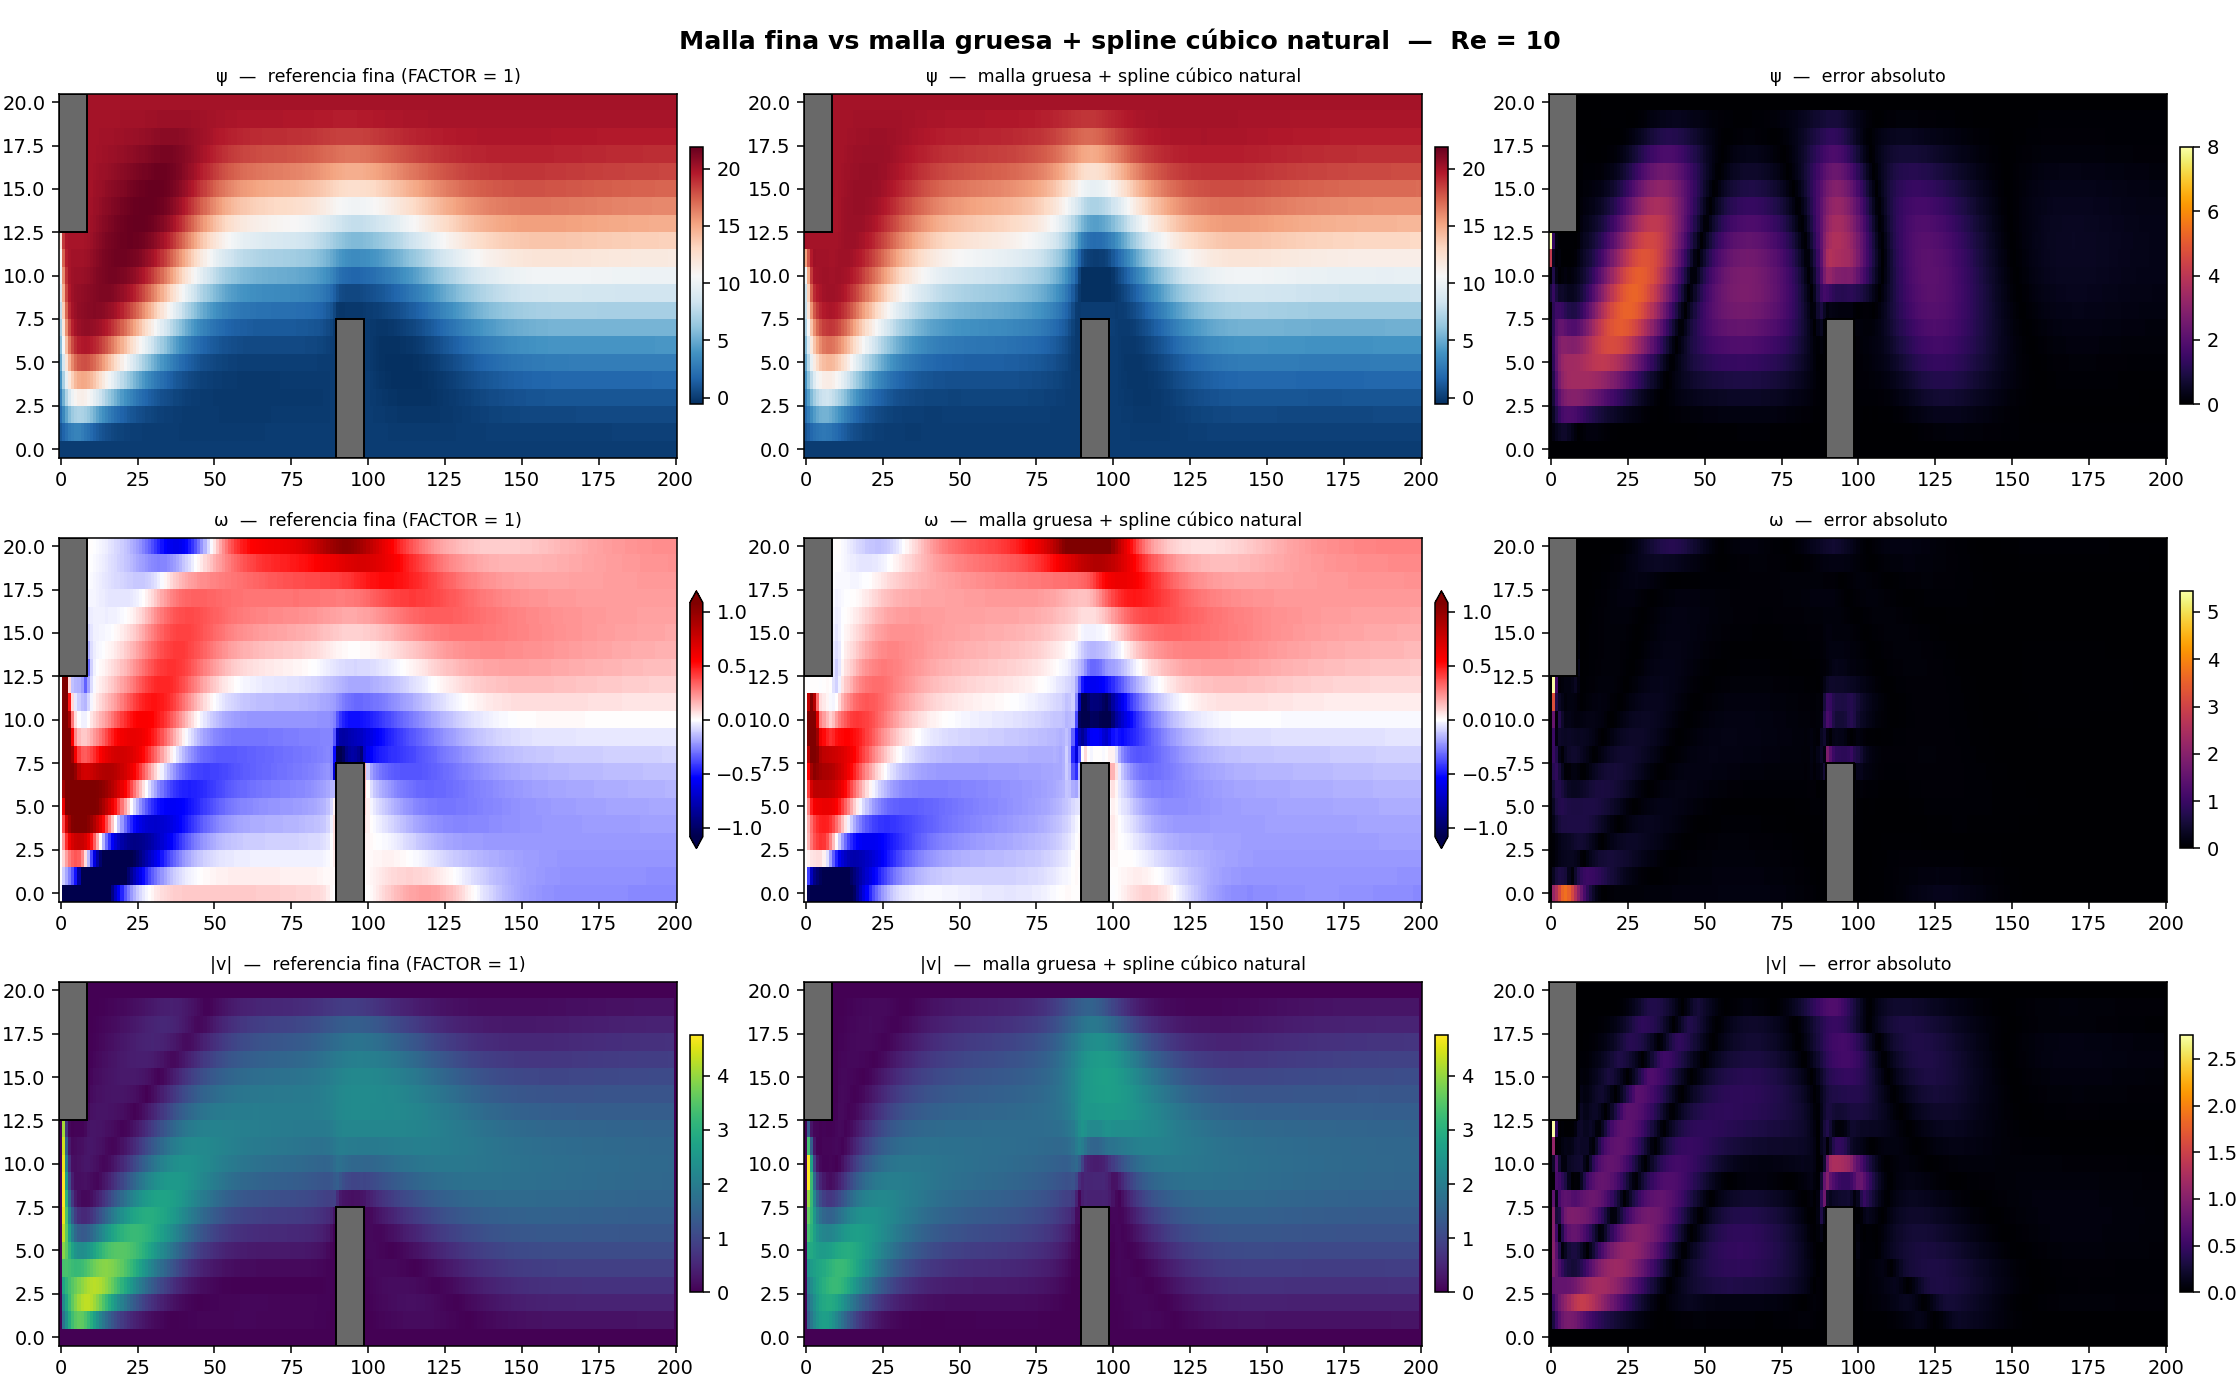
\includegraphics[width=\textwidth]{comparacion_mallas_Re10.png}
    \caption{Referencia fina (izquierda), malla gruesa reconstruida con el
    spline cúbico natural (centro) y error absoluto (derecha), para $u$,
    $w$ y $|v|$ a $Re = 10$. Cada fila comparte la escala de color entre
    referencia y reconstrucción; $w$ usa la escala simétrica recortada al
    percentil 98 para que los picos de las esquinas no aplasten el resto
    del campo.}
    \label{fig:comparacion_mallas}
\end{figure}

La reconstrucción reproduce fielmente la estructura global del flujo. En
números: la mediana del error de $u$ es $0.37$ (un $1.8\,\%$ de
$u_{\max}=20$) y la de $w$ es $0.05$; el percentil 90 del error de $u$
sube a $2.3$, concentrado en las zonas de recirculación detrás del
Bloque~1 y alrededor del Bloque~2. Un detalle revelador: excluir la franja
de redondeo geométrico junto a los bloques casi no cambia estas cifras.
Es decir, el error dominante \emph{no} proviene del spline (que es exacto
en los nodos gruesos) ni del redondeo de los bloques, sino de la propia
discretización gruesa: con $h' = 2h$ la difusión numérica del upwind se
duplica (Sección~\ref{sec:upwind}) y las recirculaciones se suavizan. Esto
confirma la limitación anticipada: la calidad la fija la malla donde se
resuelve, y el spline se limita a presentarla con suavidad en la malla
original.

\subsection{Limitaciones}

\begin{itemize}
  \item \textbf{La interpolación no añade física}: el spline presenta con
        suavidad la solución gruesa en la malla fina, pero las estructuras
        del flujo más pequeñas que el espaciado grueso $h'$ no se recuperan.
        La calidad de la solución la fija la malla donde se resolvió, no la
        malla donde se grafica.
  \item \textbf{Más difusión numérica}: la viscosidad artificial del upwind
        crece con $|v|\,h$, así que la malla gruesa suaviza los gradientes
        algo más que la fina.
  \item \textbf{Esquinas de los obstáculos}: los campos no son suaves junto
        a los bloques, y un spline puede sobrepasarse ligeramente en esas
        zonas; en las gráficas dichas regiones quedan enmascaradas por los
        obstáculos.
\end{itemize}

En conjunto, el esquema es un compromiso razonable: con $\texttt{FACTOR}=2$
el costo por iteración cae a una cuarta parte y las gráficas a $Re = 20$
siguen mostrando un campo suave y físicamente coherente en la malla
original.

%─────────────────────────────────────────────────────────────────────────────
\section{Comparación de métodos para el sistema lineal}
\label{sec:metodos-lineales}
%─────────────────────────────────────────────────────────────────────────────

Cada iteración de Newton--Raphson culmina resolviendo el sistema lineal
$J\,\Delta\mathbf{x} = -F$ (Ec.~\eqref{eq:newton_lineal}). El proyecto usa
un método \textbf{directo} (factorización LU sparse vía
\texttt{scipy.sparse.linalg.spsolve}), pero ese mismo sistema puede
resolverse con los métodos iterativos vistos en clase. En esta sección se
comparan cuatro alternativas sobre un mismo sistema, y el resultado —dos de
ellas fallan— ilustra muy bien que cada método iterativo trae hipótesis
que hay que verificar antes de usarlo.

\subsection{Montaje del experimento}

Comparar métodos sobre un sistema ya convergido sería engañoso (el residuo
es casi cero y cualquier método "gana"). En su lugar, el script
\texttt{comparacion\_metodos\_lineales.py} \textbf{congela} un paso de
Newton genuinamente difícil: toma la solución convergida para $R = 0.5$ y
evalúa $F$ y $J$ exigiéndole la física de $R = 2$. Eso produce un residuo
sustancial ($\|F\| \approx 4.5$) sobre la malla gruesa de $100\times10$:
un sistema de $2110 \times 2110$ con $13\,255$ entradas no nulas. Los
cuatro métodos resuelven exactamente ese mismo sistema:

\begin{itemize}
  \item \textbf{Directo} (\texttt{spsolve}): factorización LU sparse;
        referencia exacta.
  \item \textbf{Jacobi}: $\mathbf{x}^{(k+1)} = \mathbf{x}^{(k)} +
        D^{-1}\bigl(\mathbf{b} - J\,\mathbf{x}^{(k)}\bigr)$, con $D$ la
        diagonal de $J$; cada componente se actualiza usando solo valores
        de la iteración anterior.
  \item \textbf{Gauss--Seidel}: $(L+D)\,\mathbf{x}^{(k+1)} = \mathbf{b} -
        U\,\mathbf{x}^{(k)}$; el barrido usa los valores ya actualizados,
        resolviendo un sistema triangular por iteración.
  \item \textbf{Gradiente Conjugado} (CG): método de subespacios de Krylov
        que \emph{requiere} matriz simétrica definida positiva (SPD).
\end{itemize}

\subsection{Resultados}

\begin{center}
\begin{tabular}{lcccc}
  \toprule
  \textbf{Método} & \textbf{¿Convergió?} & \textbf{Iteraciones}
    & \textbf{Tiempo (s)} & \textbf{Error rel.\ vs directo} \\
  \midrule
  Directo (LU sparse) & sí & --- & $2.6\times10^{-3}$ & $0$ \\
  Jacobi & \textbf{no (diverge)} & 3000 (tope) & --- & $\sim 10^{131}$ \\
  Gauss--Seidel & sí & 435 & $2.1\times10^{-1}$ & $1.9\times10^{-8}$ \\
  Gradiente Conjugado & \textbf{no} & 3000 (tope) & --- & $\sim 10^{8}$ \\
  \bottomrule
\end{tabular}
\end{center}

\begin{figure}[H]
    \centering
    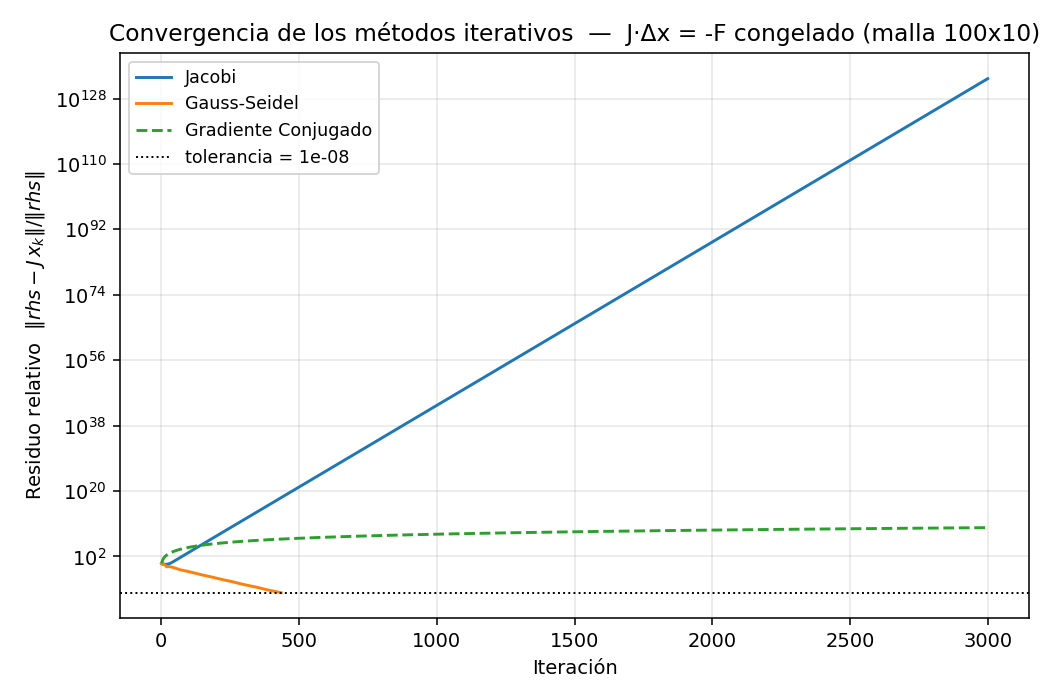
\includegraphics[width=0.75\textwidth]{convergencia_metodos_lineales.png}
    \caption{Historia de convergencia de los métodos iterativos sobre el
    sistema congelado: Jacobi diverge exponencialmente, Gauss--Seidel
    converge linealmente hasta la tolerancia en 435 iteraciones y el
    Gradiente Conjugado se estanca sin converger.}
    \label{fig:metodos_lineales}
\end{figure}

\subsection{Discusión}

\begin{itemize}
  \item \textbf{Jacobi diverge}, y el motivo es instructivo: su condición
        suficiente de convergencia es la dominancia diagonal, y $J$
        \emph{no} la cumple. En la fila de Poisson, la diagonal vale $-4$
        mientras los vecinos suman $4$ y el acoplamiento con $w$ aporta
        $h^{2}$ adicional (que con $h' = 2$ vale $4$: tan grande como la
        diagonal misma). El radio espectral de la iteración supera 1 y el
        error crece sin freno.
  \item \textbf{Gauss--Seidel sí converge} pese a la falta de dominancia:
        usar los valores ya actualizados dentro del barrido lo hace más
        robusto que Jacobi. Pero necesita 435 iteraciones, cada una con un
        sistema triangular, y termina siendo $\sim\!80$ veces más lento que
        el método directo en este tamaño.
  \item \textbf{CG no converge porque su hipótesis no se cumple}: $J$ no es
        simétrica (el término convectivo upwind y las filas de frontera
        rompen la simetría) ni definida positiva. Para sistemas no
        simétricos existen variantes de Krylov apropiadas (BiCGSTAB,
        GMRES), normalmente acompañadas de un precondicionador.
  \item \textbf{Conclusión}: para un sistema de este tamaño (miles de
        grados de libertad) y tan disperso, el método directo sparse es la
        elección correcta —milisegundos y solución exacta—. Los métodos
        iterativos se vuelven competitivos en mallas mucho mayores, donde
        la factorización LU no cabe en memoria, y aun entonces exigen
        elegir el método según las propiedades de la matriz y
        precondicionarla.
\end{itemize}

\section{Resultados}
\label{sec:resultados}

La Figura~\ref{fig:resultado_re2} muestra la solución obtenida para un número
de Reynolds \(Re = 2\), correspondiente a un régimen laminar.
Se presentan la función de corriente \(\psi\), la vorticidad \(\omega\) y el
campo de velocidades derivado de la solución numérica.

\begin{figure}[H]
    \centering
    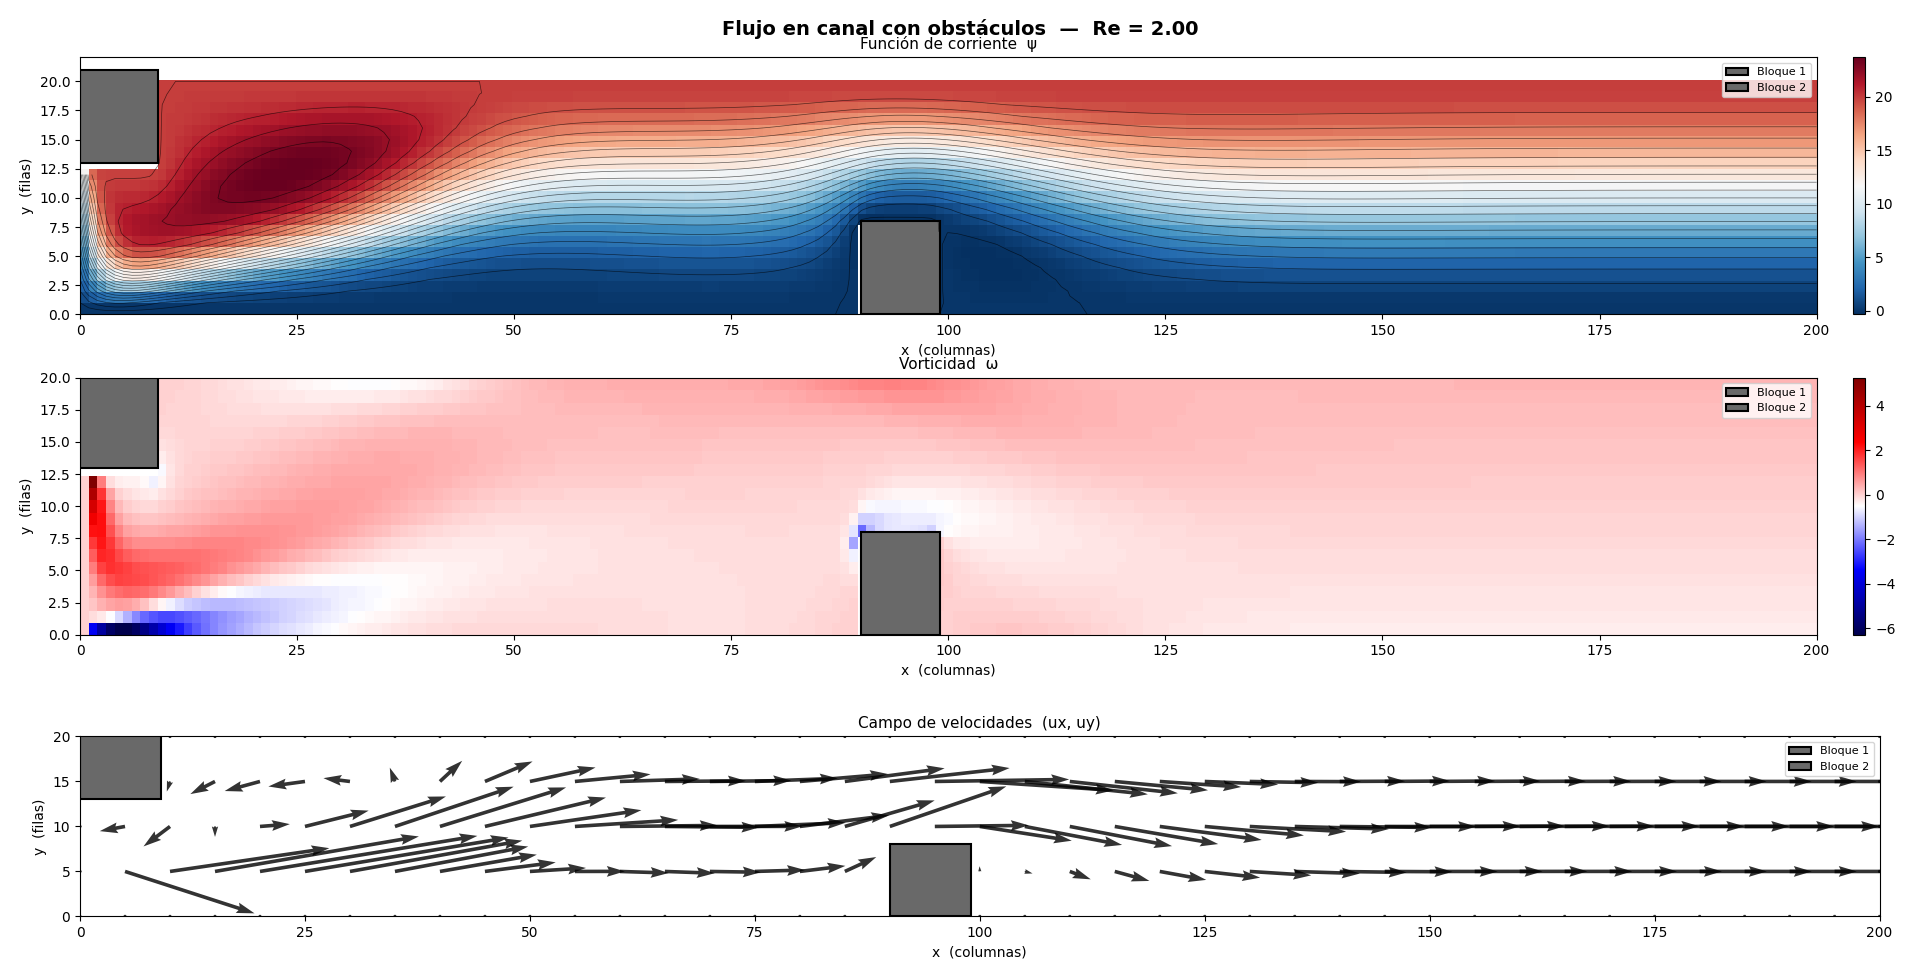
\includegraphics[width=\textwidth]{graficas.png}
    \caption{Resultados numéricos del flujo en canal con obstáculos para \(Re = 2\).}
    \label{fig:resultado_re2}
\end{figure}

\subsection*{¿Qué se ve en los resultados?}

Arriba, la función de corriente \(\psi\) dibuja las trayectorias del fluido: entra
uniforme por la izquierda, se topa con el Bloque~1 (esquina superior) y se acelera
por debajo, curvando las líneas. Luego el Bloque~2 lo vuelve a desviar, hasta que
corriente abajo todo se estabiliza otra vez.

En el centro, la vorticidad \(\omega\) enseña dónde el flujo se retuerce: mucha
actividad cerca de las paredes y las esquinas de los obstáculos, justo donde la
velocidad cambia bruscamente.

Abajo, el campo de velocidades \((u_x, u_y)\) —calculado a partir de \(\psi\)
con \(u_x = \partial\psi/\partial y\) y \(u_y = -\partial\psi/\partial x\)—
muestra un flujo laminar tranquilo, sin turbulencias ni remolinos raros.
El fluido rodea los obstáculos y vuelve a enderezarse aguas abajo.

\section {Comentarios finales}

Logramos simular un flujo viscoso 2D con obstáculos usando las ecuaciones de
Navier--Stokes en formulación \(\psi\)--\(\omega\), resueltas con diferencias
finitas, Newton--Raphson y una Jacobiana en formato sparse. El Reynolds era
bajo y la geometría simple, pero el problema nos dejó algunas reflexiones:

\begin{itemize}
    \item Las condiciones de frontera, el tratamiento de la vorticidad en paredes
          y la estabilidad del método iterativo afectan directamente a la solución
          física.
    \item Sin una estrategia de continuación en Reynolds y backtracking,
          Newton--Raphson habría sido extremadamente inestable.
    \item La matriz sparse fue lo que salvó el día: miles de grados de libertad
          que en denso no caben ni en memoria, resueltos en un tiempo razonable.
\end{itemize}

En definitiva, \textbf{incluso un problema sencillo exige cuidar cada detalle}:
formulación, discretización, álgebra lineal y ajuste numérico. Para problemas de
verdad (Reynolds altos, geometrías complejas, mallas finas) haría falta mucho más:
refinamiento adaptativo, modelos de turbulencia y esquemas más sofisticados. Ahí
se ve el real potencial de la CFD.

\section{Bibliografía}

\begin{thebibliography}{9}

\bibitem{landau}
Rubin H. Landau, Manuel José Páez y Cristian C. Bordeianu,
\textit{Computational Problems for Physics: With Guided Solutions Using Python},
Wiley-VCH, 2018.

\bibitem{ecuaciones}
\textit{Ecuaciones diferenciales: Para estudiantes de Ciencias e Ingenierías},
Programa Editorial Universidad del Valle,
2014.


\bibitem{calculo}
\textit{Cálculo avanzado: Cálculo en varias variables, teoría, problemas propuestos y resueltos, utilización de Mathematica},
Programa Editorial Universidad del Valle,
2018.

\end{thebibliography}

\end{document}